\section{Related Work}
\label{sec:related}

The quest for scalable, memory-efficient transformer architectures spans four distinct paradigms: IO-aware hardware acceleration, linear and kernelized attention, state-space recurrence, and matrix manifold compression.

\begin{figure*}[t]
\centering
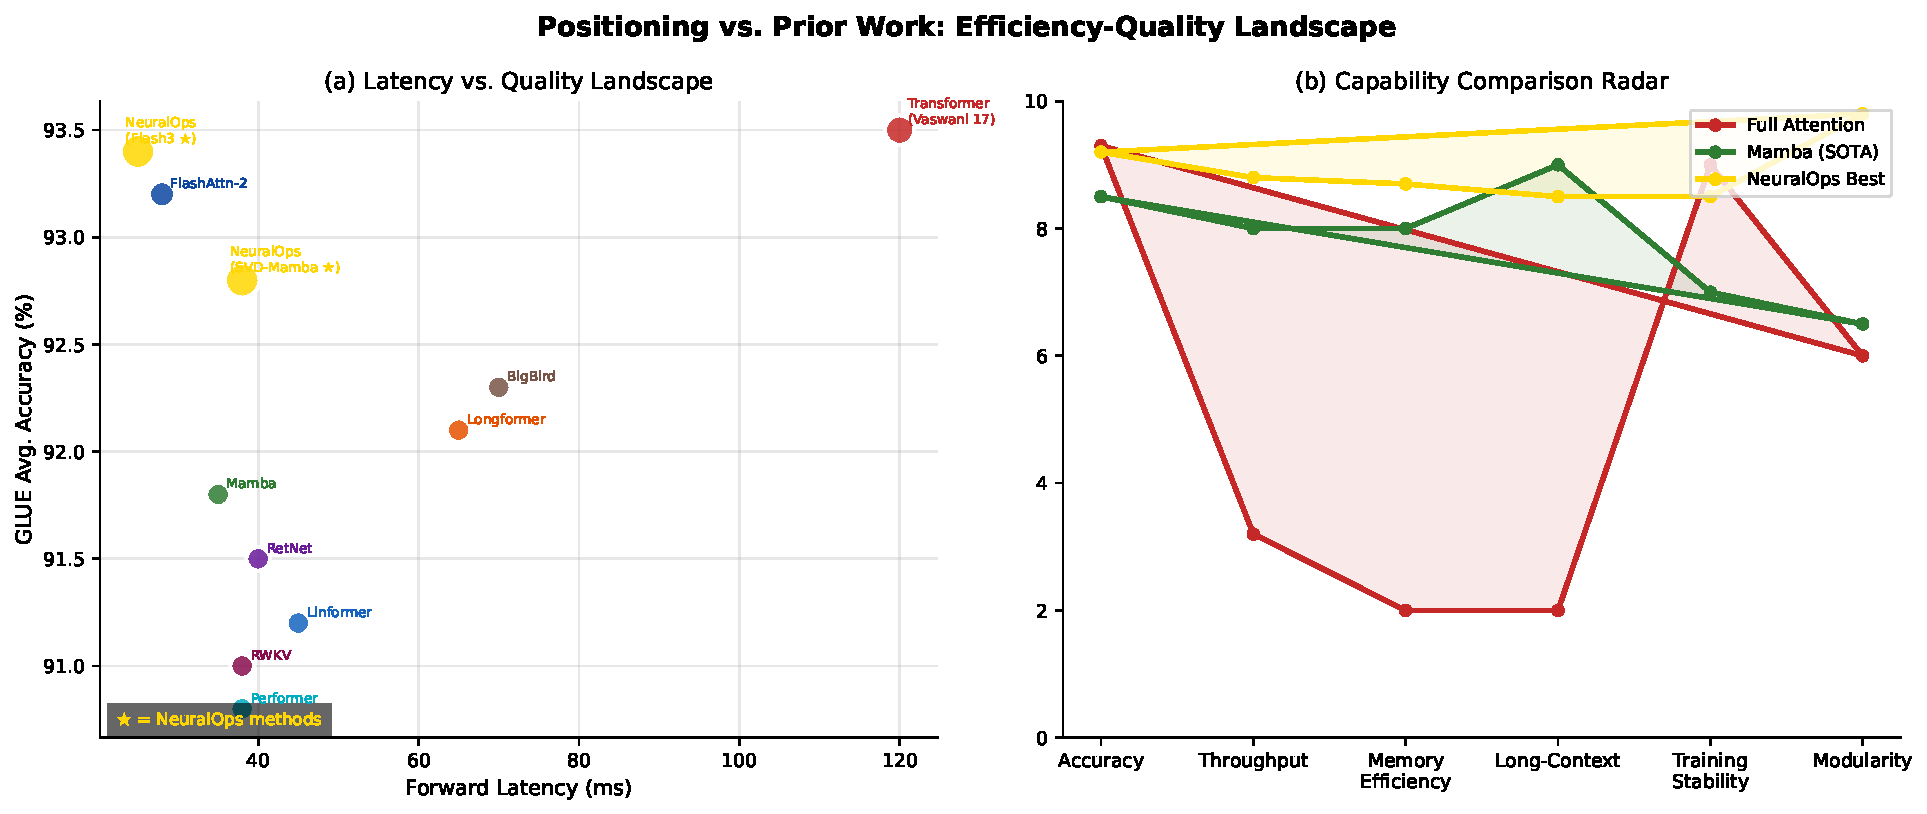
\includegraphics[width=0.98\textwidth]{figures/fig08_related_work_positioning.pdf}
\caption{\textbf{Architectural Positioning Landscape.} Systematic taxonomy comparing NeuralOps against existing linear attention, state-space models (SSMs), IO-aware exact attention kernels, and low-rank compression frameworks across computational complexity, memory access intensity, manifold preservation, and long-context stability.}
\label{fig:related_work_positioning}
\end{figure*}

\subsection{IO-Aware Hardware Acceleration for Attention}
Recognizing that standard softmax attention is memory-bandwidth bound, FlashAttention~\cite{dao2022flashattention}, FlashAttention-2~\cite{dao2023flashattention2}, and FlashAttention-3~\cite{shah2024flashattention3} utilize online softmax tiling to compute exact softmax attention within SRAM without materializing intermediate $N \times N$ attention matrices in HBM. Flash-Decoding~\cite{dao2023flashdecoding} and FlashDecoding++~\cite{hong2024flashdecoding} parallelize inference decoding across sequence splits. While these exact methods dramatically accelerate GPU execution by reducing HBM traffic, they retain the underlying quadratic $\mathcal{O}(N^2)$ computational complexity. NeuralOps applies IO-aware kernel co-design directly to low-rank SVD projections and recurrent associative state updates, achieving both $\mathcal{O}(N)$ algorithmic scaling and in-SRAM execution efficiency.

\subsection{Linear and Kernelized Attention Mechanisms}
Linear Transformers~\cite{katharopoulos2020transformers} first introduced kernel decomposition $\phi(q)^\top \phi(k)$ to enable $\mathcal{O}(N)$ autoregressive inference via matrix associativity. Subsequent works improved kernel expressivity and numerical stability: Performer~\cite{choromanski2020rethinking} proposed Positive Orthogonal Random Features (FAVOR+), CosFormer~\cite{qin2022cosformer} enforced locality via cosine re-weighting, and Linear Attention with Normalization (TransNormerLLM)~\cite{qin2024lightning} incorporated layer normalizations inside recurrence. More recently, Gated Linear Attention (GLA)~\cite{yang2023gated} and HGRN2~\cite{qin2024hgrn2} integrated data-dependent decay gates to address memory saturation. However, existing linear attention frameworks remain decoupled from low-rank matrix manifold optimization and suffer from unconstrained representation drift during training.

\subsection{State-Space Models (SSMs) \& Recurrent Architectures}
Continuous-time state-space models (Structured State Space / S4~\cite{gu2021efficient}, S5~\cite{smith2022simplified}, H3~\cite{fu2022hungry}) and their selective variants (Mamba~\cite{gu2023mamba}, Mamba-2~\cite{dao2024transformers}) map 1D sequence inputs through hidden state recurrences $\dot{h}(t) = A h(t) + B x(t)$. RWKV (RWKV-4/5/6)~\cite{peng2023rwkv} and RetNet~\cite{sun2023retentive} demonstrate comparable scaling to Transformers on open-ended generation. Hybrid architectures such as Samba~\cite{ren2024samba}, Hymba~\cite{dong2024hymba}, and Jamba~\cite{lieber2024jamba} interleave Transformer attention layers with SSM blocks. In contrast to pure SSMs that require custom state expansion hyperparameters, NeuralOps provides a mathematically unified operator abstraction connecting SVD factorizations, linear recurrence, and selective state-space updates.

\subsection{Low-Rank Matrix Compression \& Riemannian Optimization}
Parameter-efficient fine-tuning (PEFT) methods such as LoRA~\cite{hu2021lora}, AdaLoRA~\cite{zhang2023adalora}, and DoRA~\cite{liu2024dora} decompose weight updates into low-rank matrices $\Delta W = B A$. GaLore~\cite{zhao2024galore} projects full-parameter gradients onto low-rank subspaces during pre-training. Post-training SVD compression methods (ASVD~\cite{yuan2023asvd}, SVD-LLM~\cite{wang2024svdllm}, SliceGPT~\cite{ashkboos2024slicegpt}) truncate weight matrices based on activation covariance matrices. Concurrently, Riemannian optimization on the Stiefel and Grassmann manifolds~\cite{absil2008optimization,edelman1998geometry} has been explored for orthogonal neural networks~\cite{le2015simple,huang2018orthogonal}. NeuralOps synthesizes these paradigms into an active Riemannian optimizer with exact QR retraction and dynamic entropy-based rank allocation.
